\section{Motivation}
\begin{frame}
    \begin{itemize}
        \item HTTP/3 \cite{rfc9114} commands 20\% of internet traffic worldwide~\cite{cloudflare2024}
        \item Uses QUIC~\cite{rfc9000} as its L4 protocol
        \item QUIC throughput is not able to match TCP with increasing bandwidth~\cite{Zhang_2024}
        \item Packet I/O is QUIC's largest bottleneck in terms of its maximum achievable throughput \cite{quic_on_the_highway}
    \end{itemize}

    \textbf{XDP offers a remedy}
\end{frame}

% - Start off by talking about motiviation
%     - HTTP/3 commands 20\% of internet traffic worldwide and projected to grow? (this is why it's important)
%     - It has been shown to be slower than TCP on high-bandwidth networks (the problem)
%     - So we have to figure out a way to make it faster
%     - The biggest bottleneck in QUIC is packet I/O
%     - So let's explore one of the ways to reduce packet I/O -- i.e. XDP

\section{XDP Primer}
\begin{frame}
    \begin{itemize}
        \item XDP is a native Linux hook point for eBPF bytecode to run
        \item One of the earliest points the OS can access a packet
        \item Decide on an action for each packet
        \begin{itemize}
            \item XDP\_DROP
            \item XDP\_PASS
            \item XDP\_REDIRECT
            \item XDP\_ABORTED
            \item XDP\_TX
        \end{itemize}
    \end{itemize}
\end{frame}

\section{XDP Primer}
\begin{frame}
    \begin{itemize}
        \item AF\_XDP is an address family in Linux similar to AF\_INET or AF\_INET6
        \item It works with XDP and allows a packet skip the network stack
        \item Helps avoid costly per packet processing
    \end{itemize}
    \begin{figure}
        \centering
        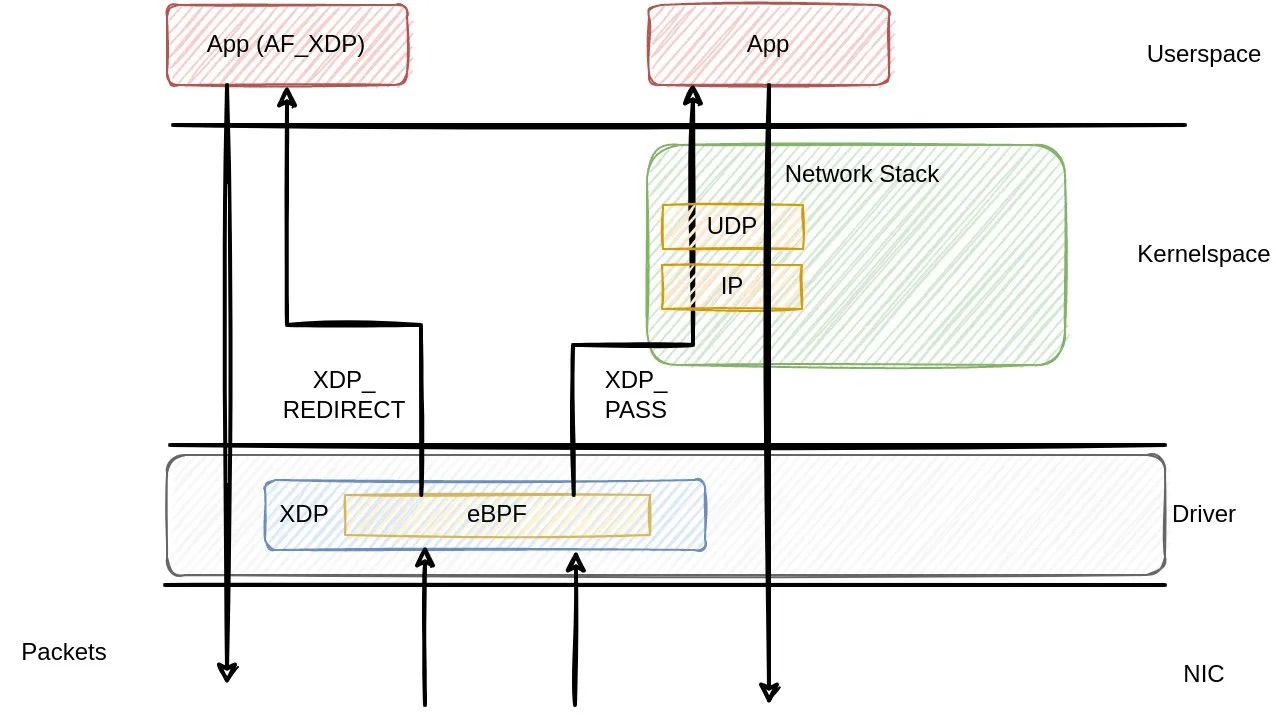
\includegraphics[width=.75\textwidth]{pics/af_xdp_diagram.jpeg}
        \nocite{af_xdp_image}
        \label{fig1}
    \end{figure}
\end{frame}

\section{AF\_XDP Primer}
\begin{frame}
    \begin{itemize}
        \item AF\_XDP uses UMEM with tx, rx, completion, and fill rings
        \item Each ring is single producer, single consumer
        \item Avoids locking contention
        \item Need a single system call to trigger multi-packet sends
    \end{itemize}
    \begin{figure}
        \centering
        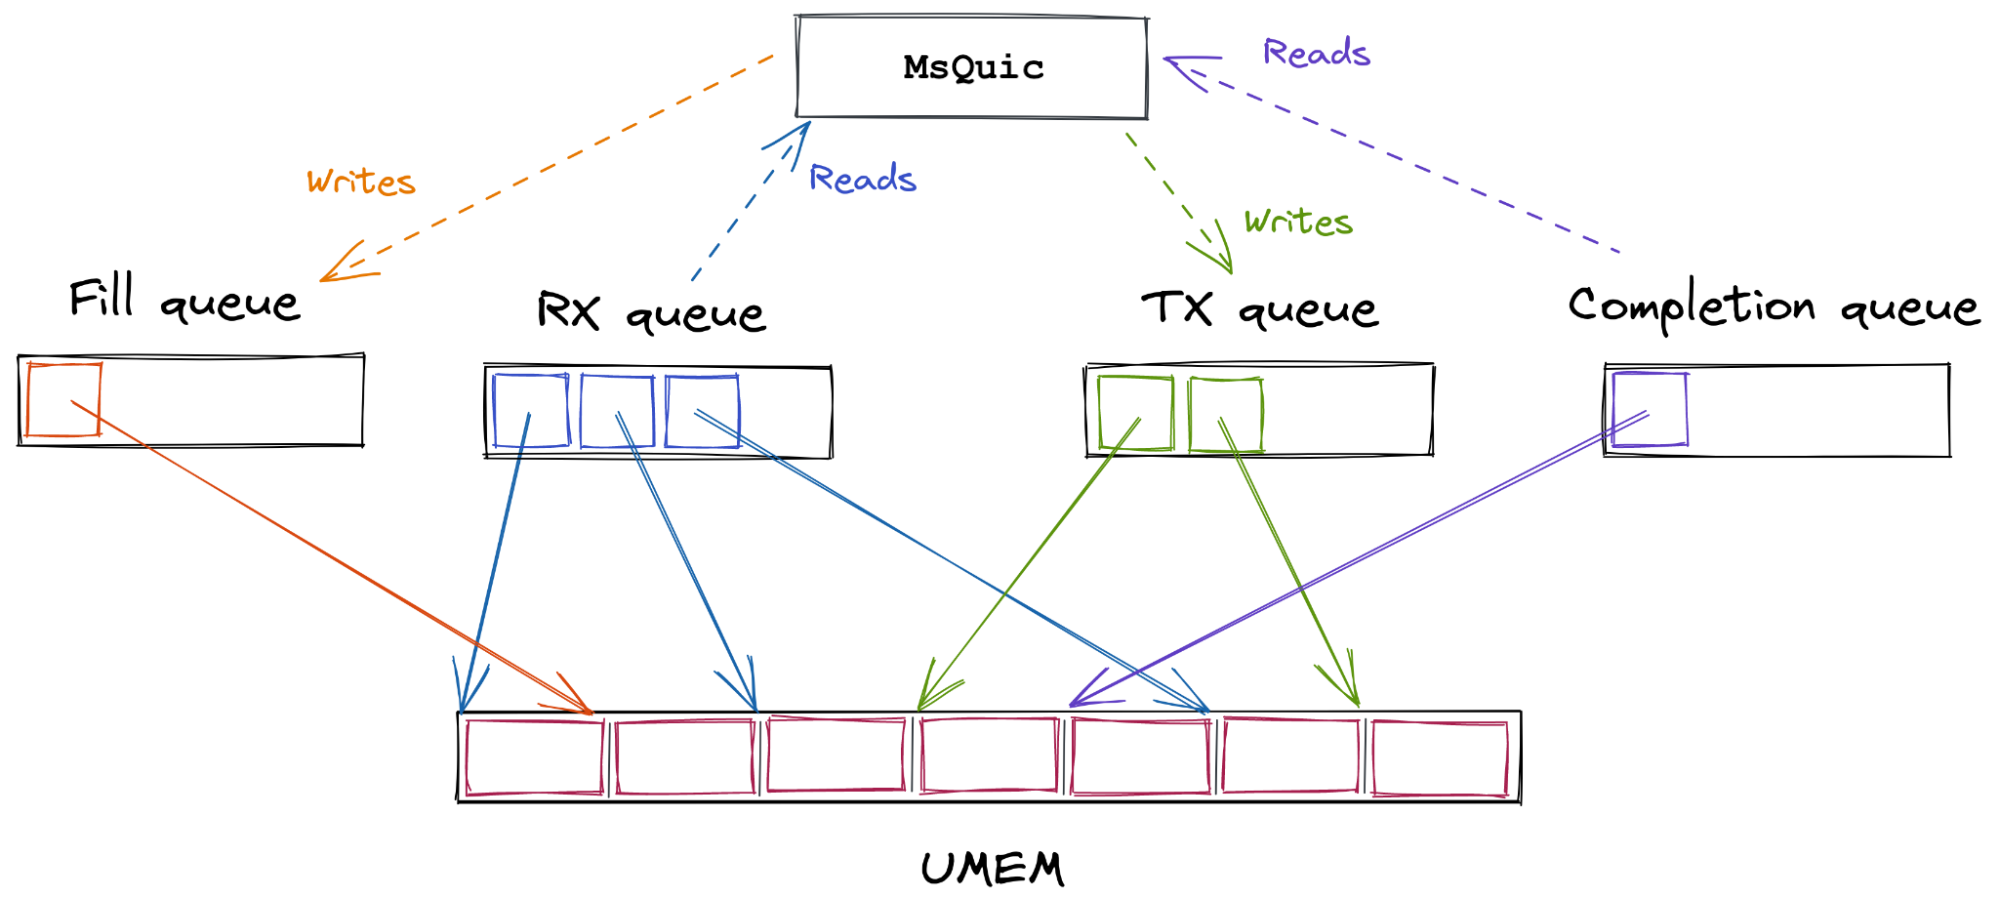
\includegraphics[width=.75\textwidth]{pics/umem.png}
        \nocite{cloudflare_af_xdp_cookie}
        \label{fig2}
    \end{figure}
\end{frame}

% - Then give brief introductions to XDP and QUIC
%     - QUIC is an L4 protocol, similar to TCP, which runs in userspace. This means packets must go through the network stack to reach the protocol. The network stack may waste cycles adding metadata to your packet that you don't need. AF_XDP allows you to get the packet at the earliest possible point.
%     - AF_XDP lets you skip the Linux network stack
%     - XDP is a hook in the kernel which allows you to process handle a packet at the 
%     earliest possible time. It is a _native_ kernel feature, which means you can use
%     it for many possible applications.

\section{Approach}
\begin{frame}
    \begin{itemize}
        \item Patch MsQuic \cite{msquic_github} interop runner to support AF\_XDP
        \item Run throughput tests in a client-server topology
        \item Generate Flame Graphs \cite{gregg_flamegraph} to identify bottlenecks
    \end{itemize}
    \begin{figure}
        \centering
        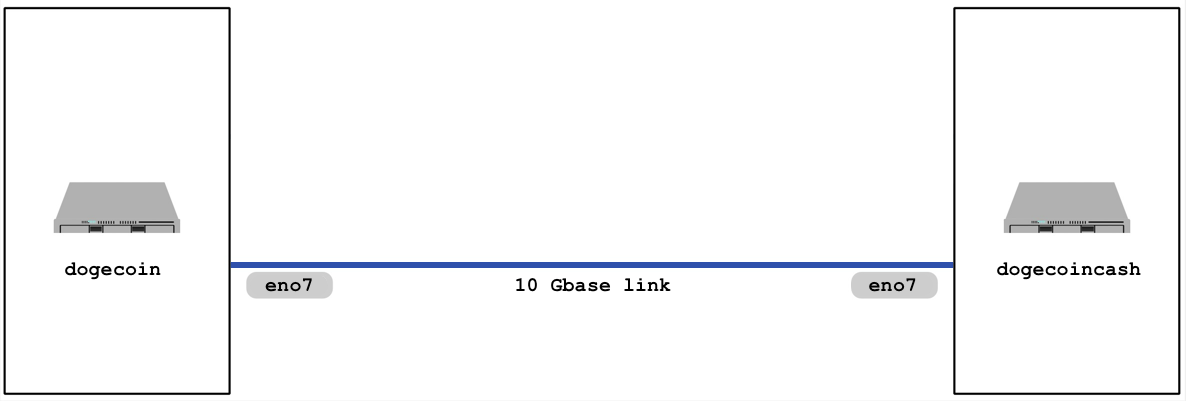
\includegraphics[width=.75\textwidth]{pics/network-topology.png}
        \nocite{network-topology}
        \label{fig3}
    \end{figure}
\end{frame}

\section{Optimization}
\begin{frame}
    Datapath long initialization time (3s perf trace) optimized by creating UMEM for only one queue on one interface
    \begin{figure}
        \centering
        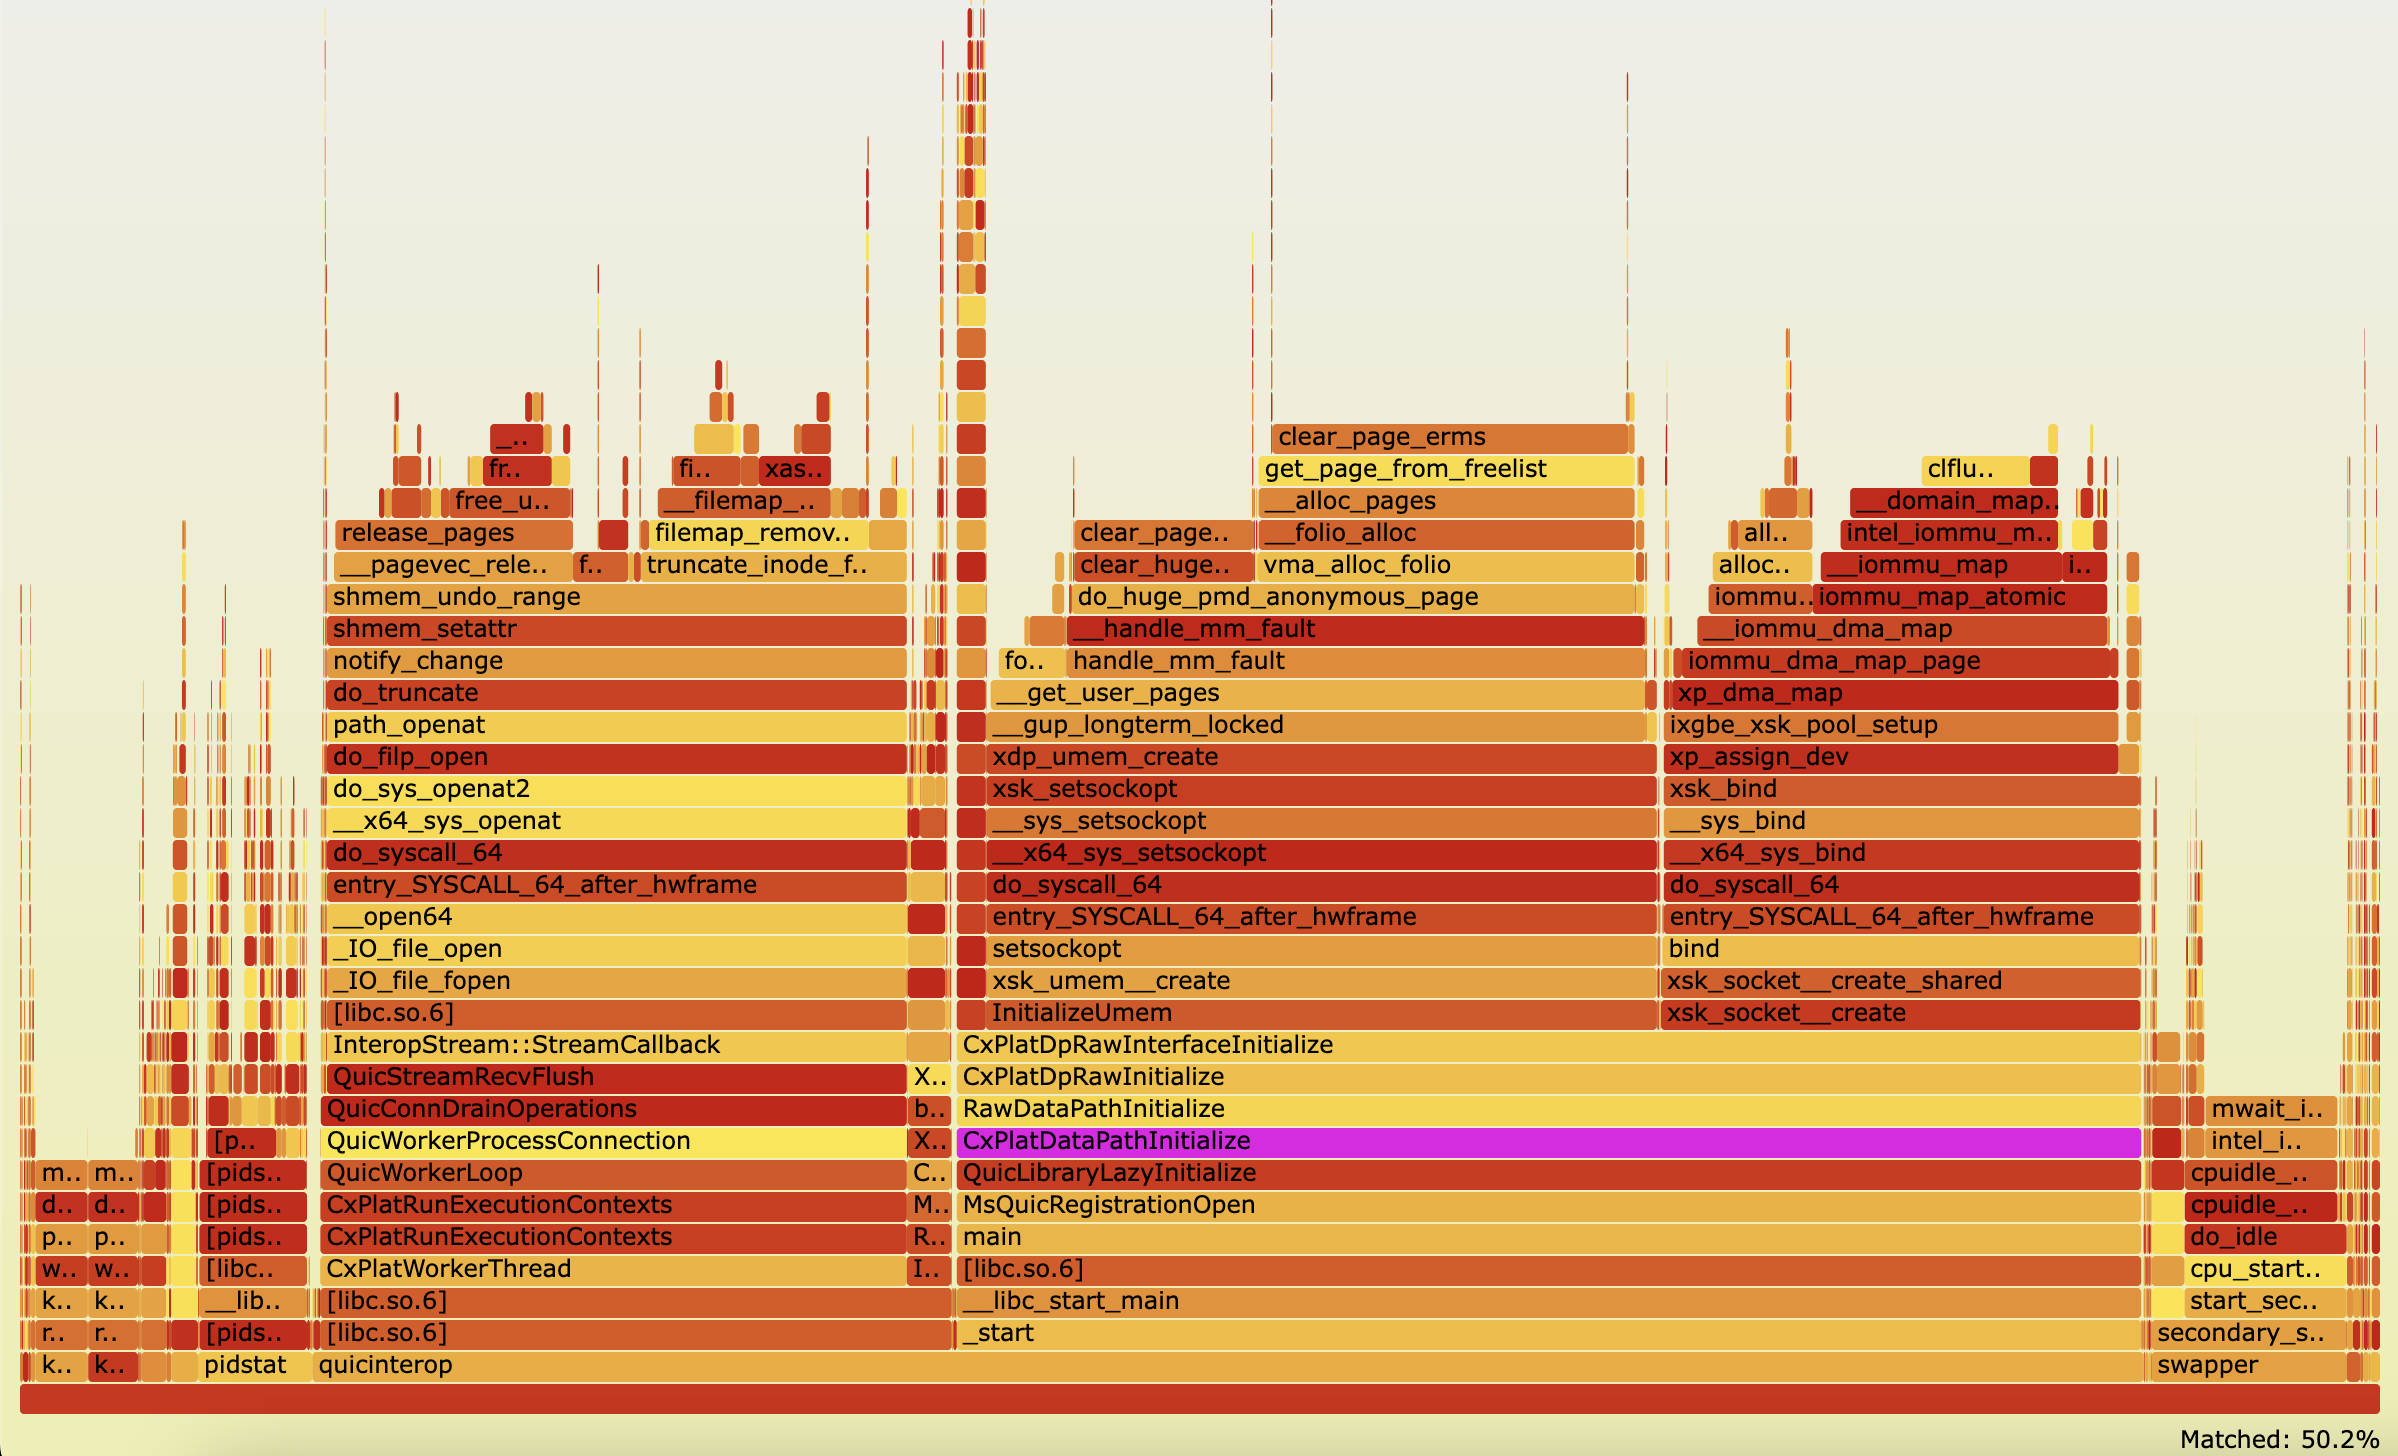
\includegraphics[width=1\textwidth]{pics/DataPathInitialize_beforeOpt.png}
        \label{fig31}
    \end{figure}
\end{frame}

\section{Optimization}
\begin{frame}
    \begin{figure}
        \centering
        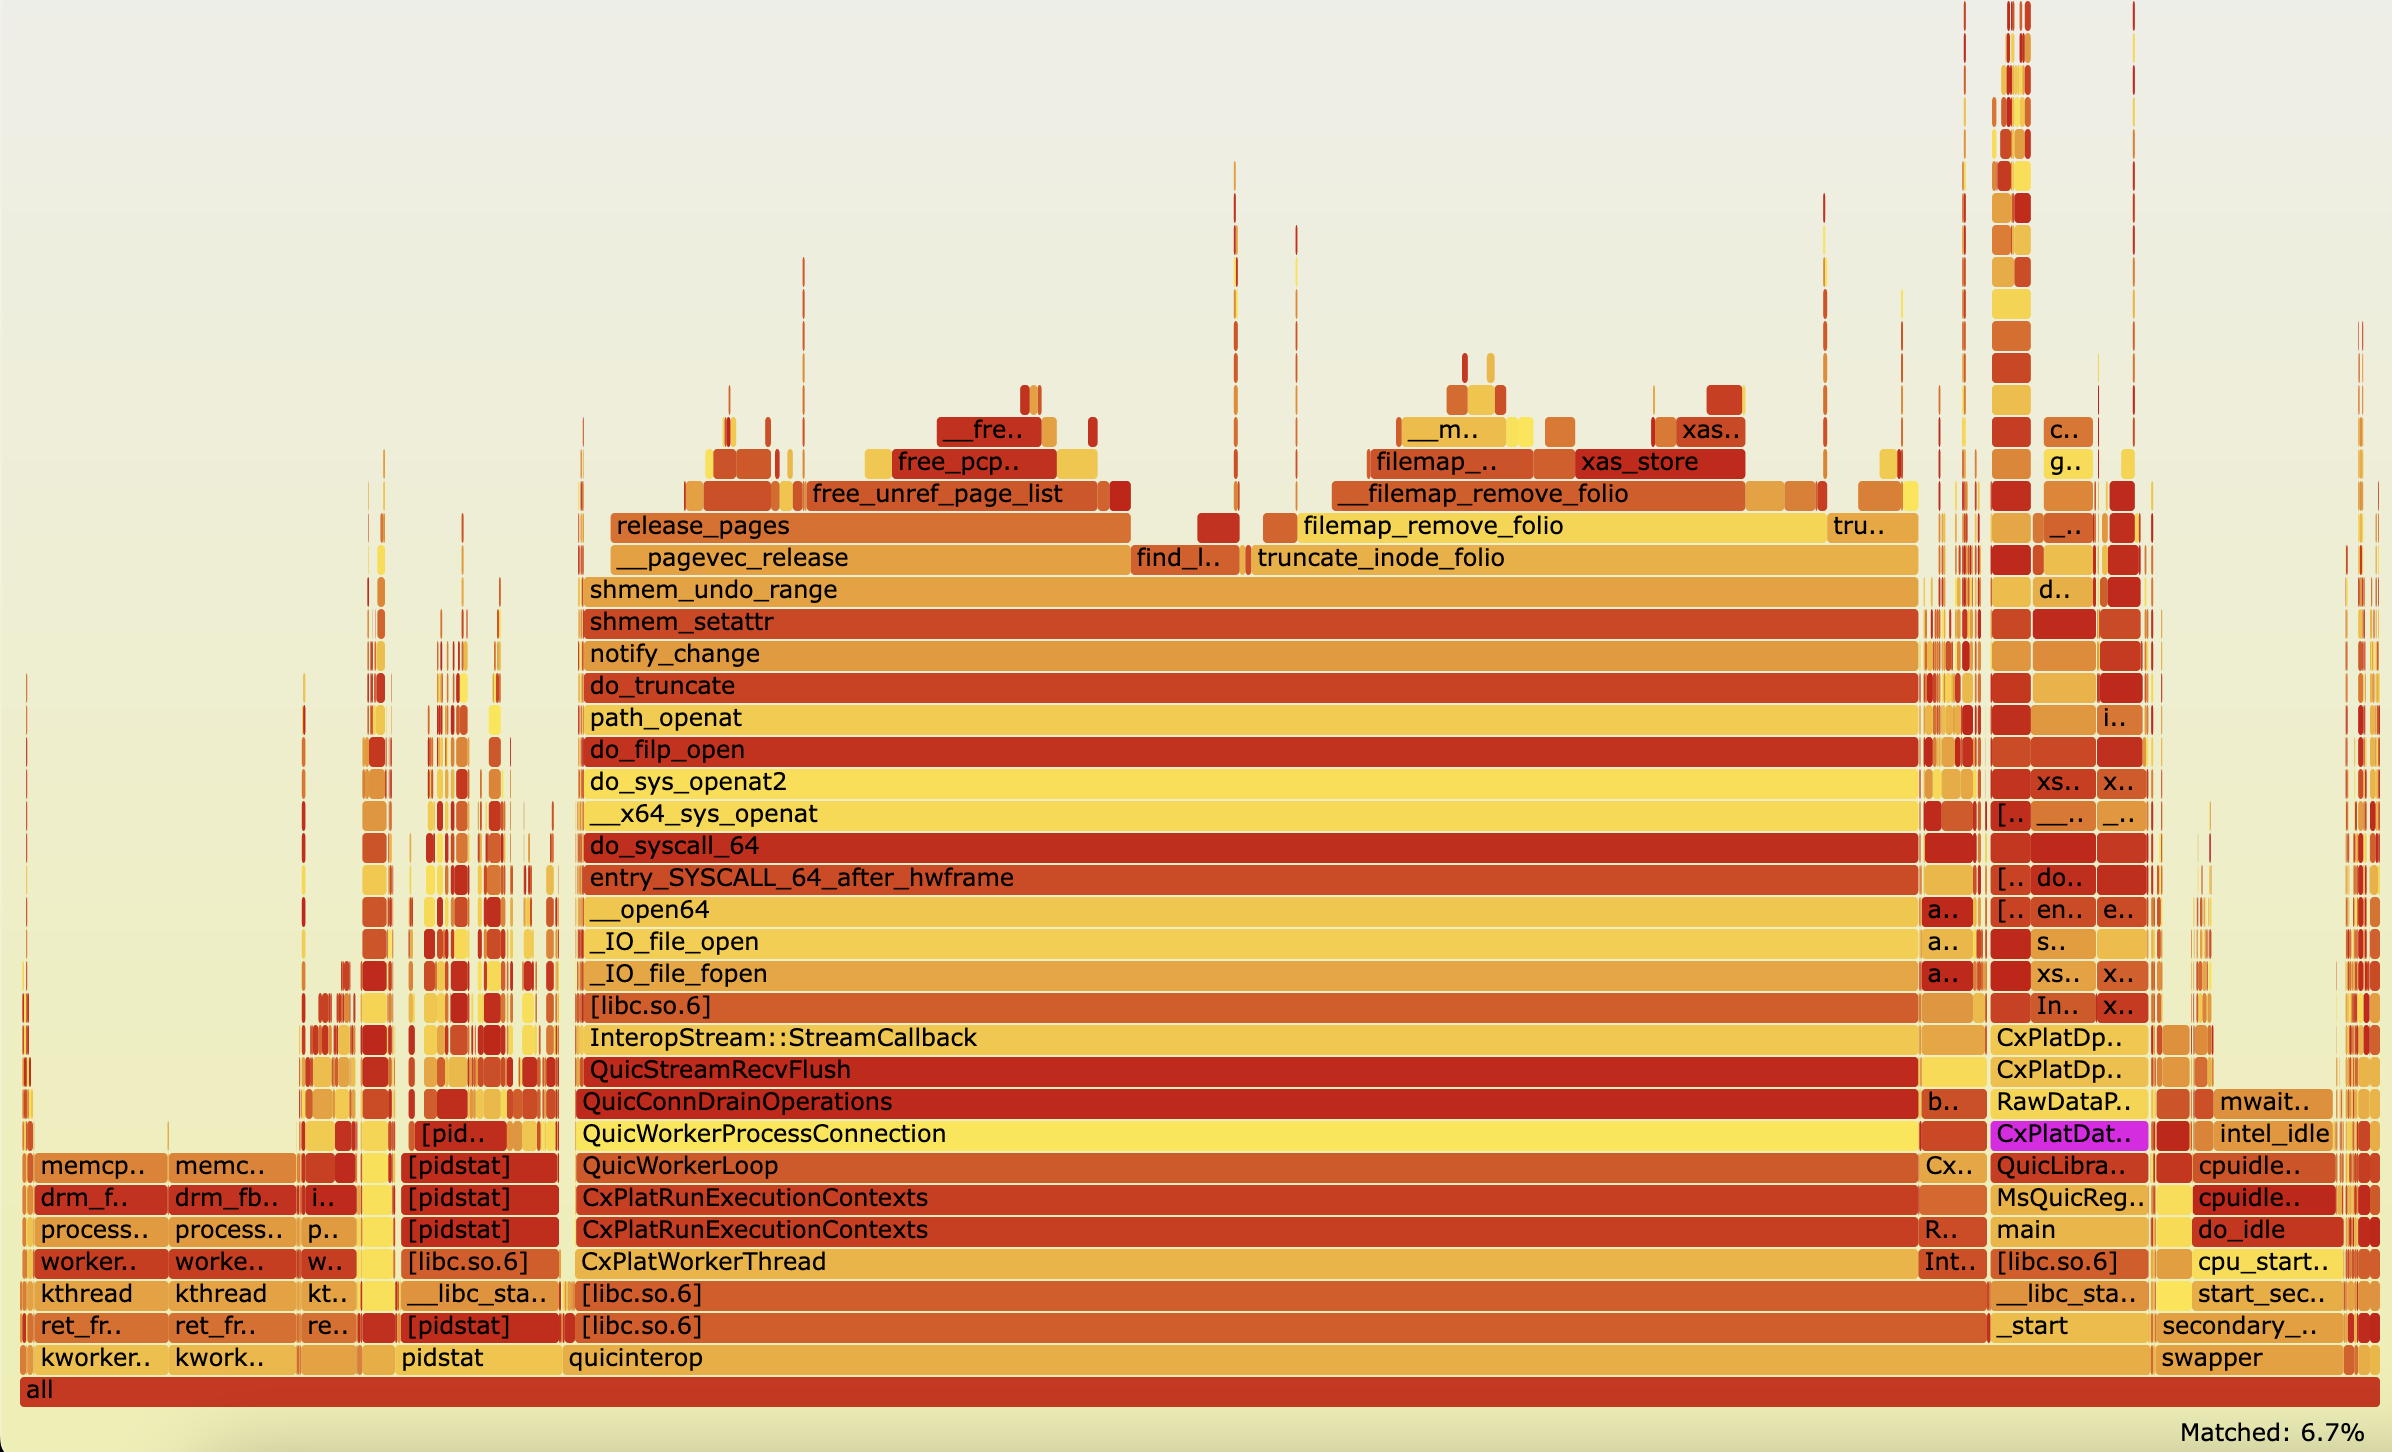
\includegraphics[width=1\textwidth]{pics/DataPathInitialize_afterOpt.png}
        \label{fig32}
    \end{figure}
\end{frame}

\section{Measurements}
\begin{frame}
    \begin{itemize}
        \item Start with baseline MsQuic datapath (recvmmsg+GRO)
        \item Switch datapath to AF\_XDP XDP\_SKB mode
    \end{itemize}
    \begin{figure}
        \centering
        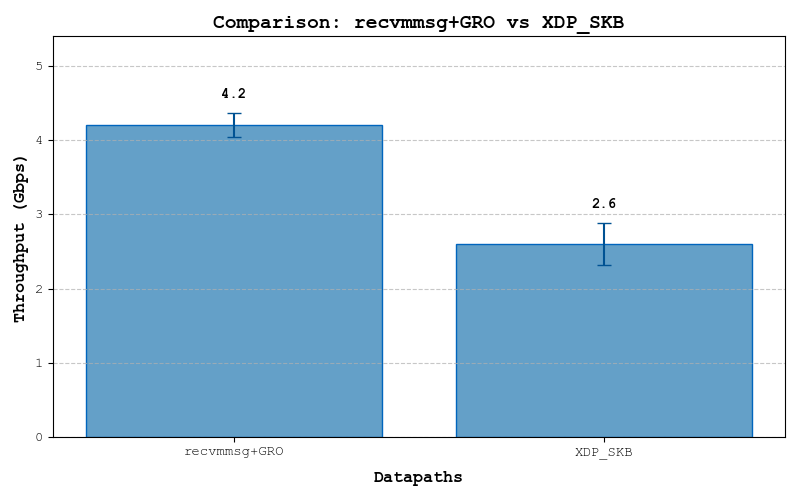
\includegraphics[width=.75\textwidth]{pics/two_dogecoin.png}
        \label{fig4}
    \end{figure}
\end{frame}

\section{Measurements}
\begin{frame}
    \begin{itemize}
        \item Move the XDP hook point closer to the driver with XDP\_DRV
        \item No longer constructing sk\_buffs, so less overhead per packet
    \end{itemize}
    \begin{figure}
        \centering
        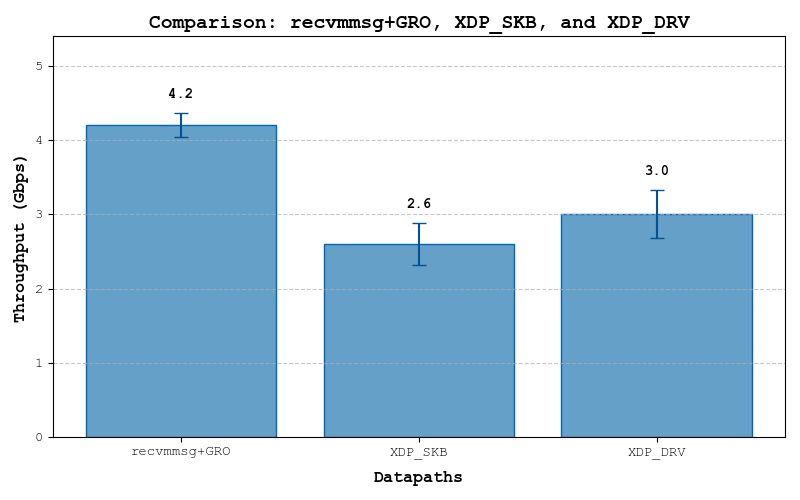
\includegraphics[width=.75\textwidth]{pics/three_dogecoin.png}
        \label{fig5}
    \end{figure}
\end{frame}

\section{Measurements}
\begin{frame}
    \begin{itemize}
        \item Eliminate an unnecessary additional copy to userspace with XDP\_ZEROCOPY
        \item NIC now DMAs packet directly into UMEM frame
    \end{itemize}
    \begin{figure}
        \centering
        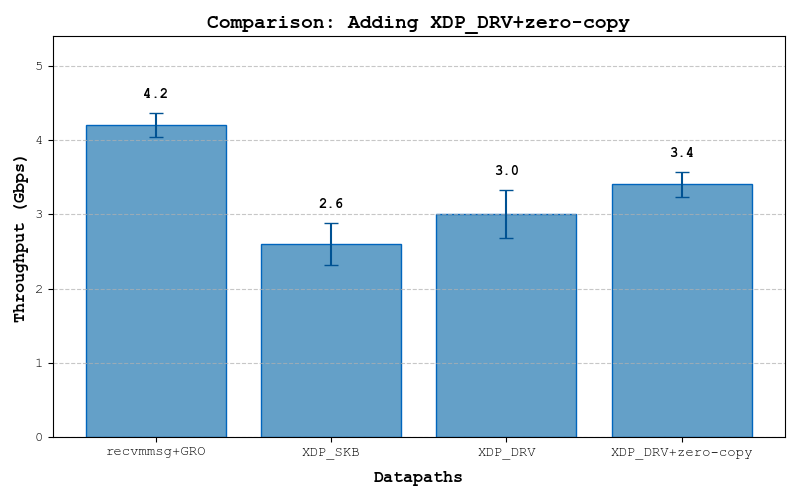
\includegraphics[width=.75\textwidth]{pics/four_dogecoin.png}
        \label{fig6}
    \end{figure}
\end{frame}

\section{Measurements}
\begin{frame}
    \begin{itemize}
        \item GRO is the main reason the default datapath is so fast
        \item Can we use GRO with XDP?
    \end{itemize}
    \begin{figure}
        \centering
        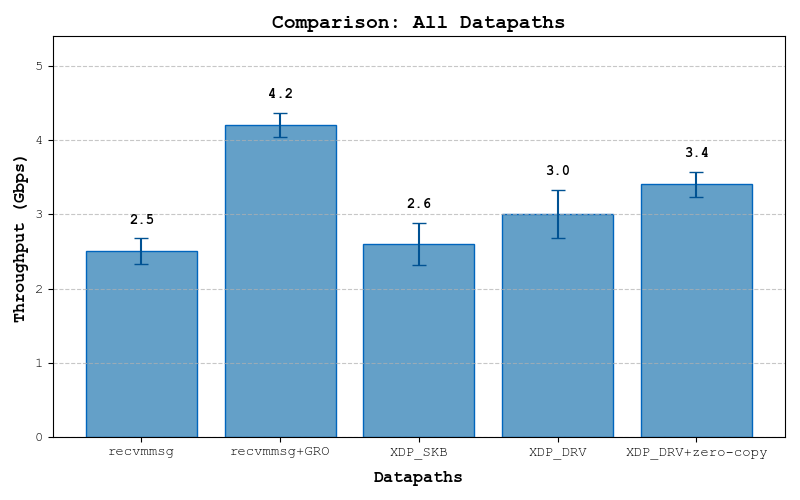
\includegraphics[width=.75\textwidth]{pics/five_dogecoin.png}
        \label{fig7}
    \end{figure}
\end{frame}

\section{GRO for XDP}
\begin{frame}
    \begin{itemize}
        \item Fragmentation with XDP now supported by some NIC drivers \cite{torvalds2021xdp}
        \item \texttt{rx-gro-hw} with XDP\_DRV or GRO with XDP\_SKB when HW offload not available
    \end{itemize}
    \begin{figure}
        \centering
        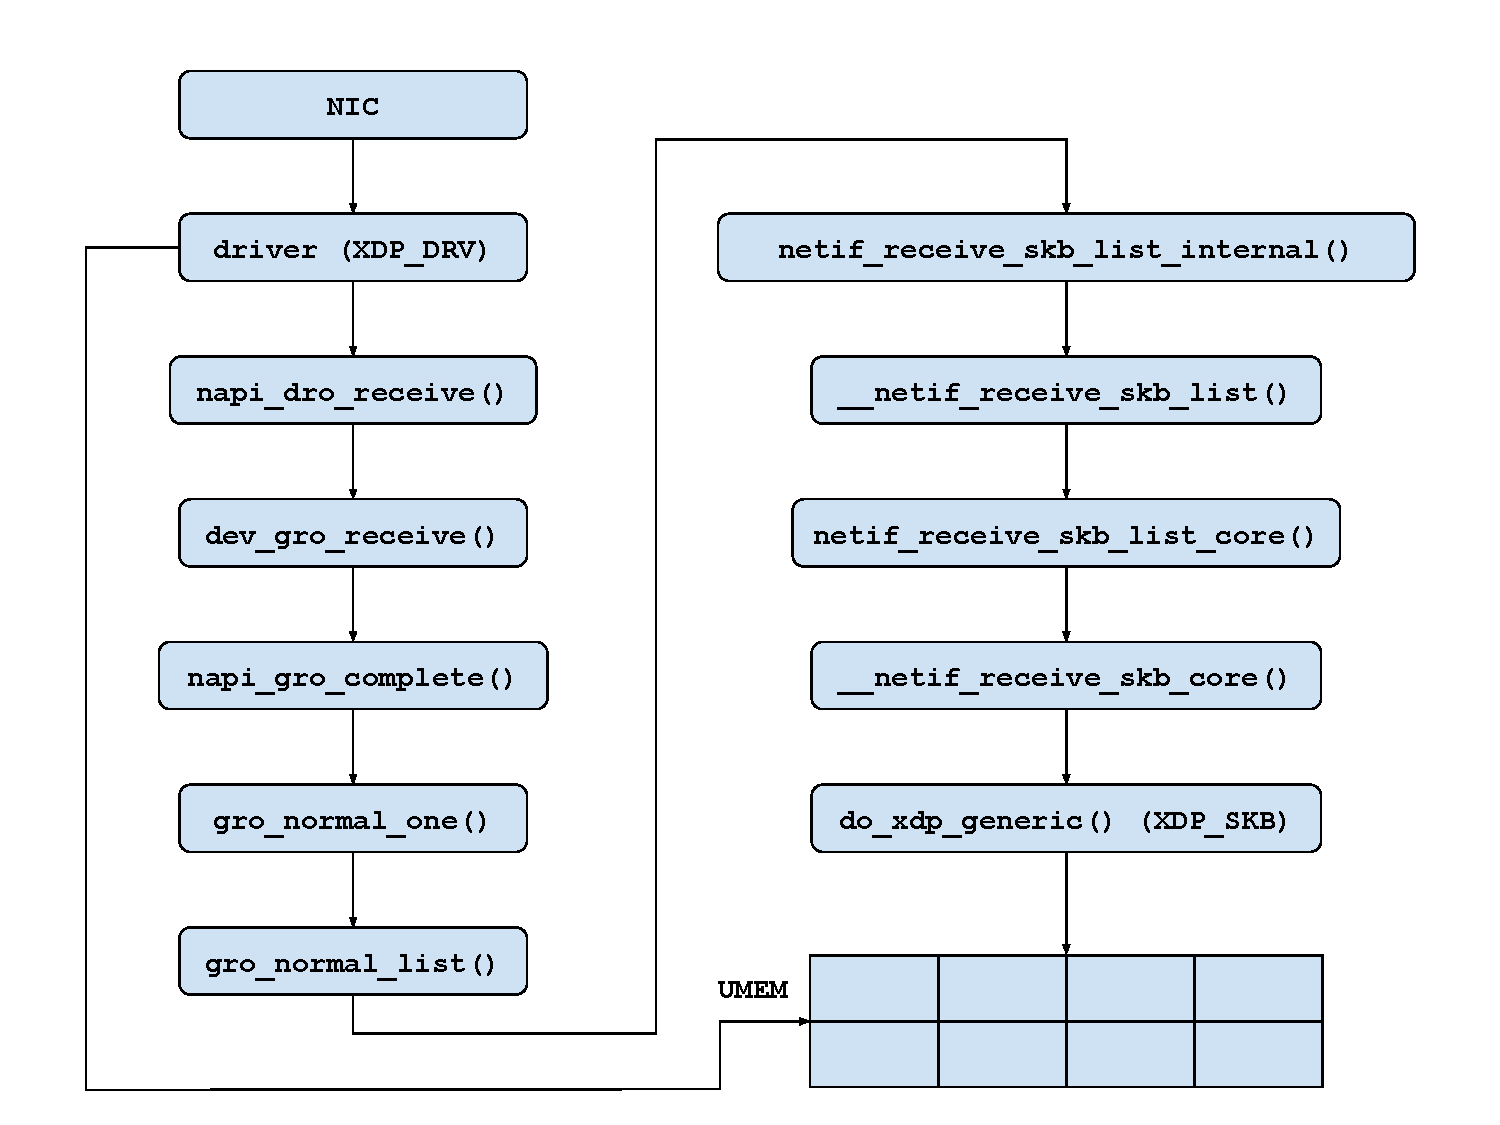
\includegraphics[width=.75\textwidth]{pics/gro_offload.pdf}
        \label{fig8}
    \end{figure}
\end{frame}

\section{Related Work}
\begin{frame}
    \begin{itemize}
        \item DPDK \cite{dpdk} enables kernel bypass and allows application to connect directly to the NIC, reducing kernel overhead
        \item lxin-quic \cite{lxin_quic} brings QUIC into the kernel, reducing context switches and copying between kernel and userspace
        \item \textit{QUIC Performance Improvements Using Socket Optimizations and Kernel Bypass}~\cite{spaeth2023} investigates methods to improve QUIC performance by means
        of patching MsQuic with DPDK and using socket optimizations
    \end{itemize}
    % \begin{figure}
    %     \centering
    %     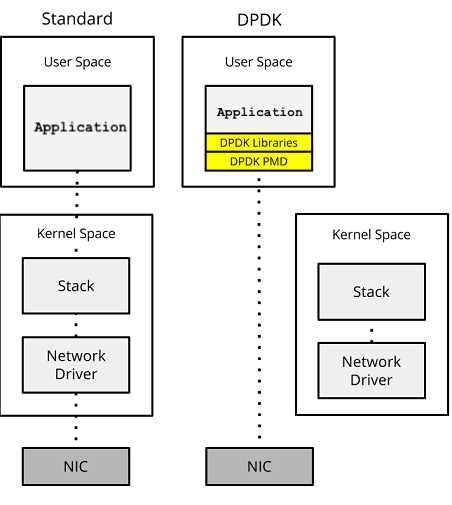
\includegraphics[width=.75\textwidth]{pics/dpdk.png}
    %     \label{fig81}
    %     \nocite{donato2018dpdk}
    % \end{figure}
\end{frame}

\section{Next Steps}
\begin{frame}
    \begin{itemize}
        \item Investigate AF\_XDP latency with clock-sychronized splitter and client to measure packet latency based on timing of arrived packets
        \item Create taxonomy for QUIC optimizations in terms of implementation complexity, performance improvement potential, unwanted side effects, flexibility, privilege level usage, and dynamic vs. static loading
    \end{itemize}
    \begin{figure}
        \centering
        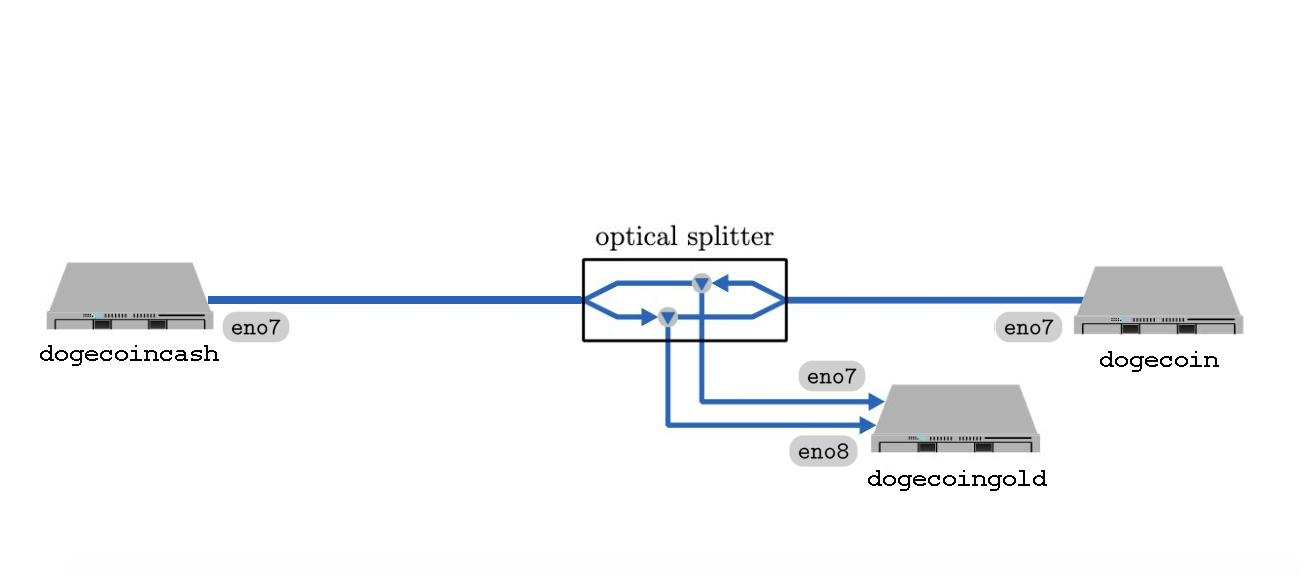
\includegraphics[width=.75\textwidth]{pics/latency_topology.pdf}
        \label{fig9}
    \end{figure}
\end{frame}

\section{Conclusion}
\begin{frame}
    \begin{itemize}
        \item AF\_XDP is not able to achieve a higher throughput over recvmmsg()+GRO
        \item XDP fragmentation support enables AF\_XDP+GRO to further increase performance
        \item AF\_XDP skipping the network stack may benefit latency
        \item AF\_XDP represents one of many methods to reduce packet IO, each with its strengths and weaknesses
    \end{itemize}
\end{frame}

% \section{FEC Primer}
% \begin{frame}
%     % \frametitle{What is FEC}
%     \begin{itemize}
%         \item Protect QUIC stream and datagram frames
%         \item Trade bandwidth for reliability
%         \item Send redundant data
%         \item Reconstruct lost information with repair symbols
%     \end{itemize}
%     \begin{figure}
%         \centering
%         \includegraphics[width=.75\textwidth]{pics/source_repair2}
%         \label{fig2}
%     \end{figure}
% \end{frame}

% \section{FEC Primer}
% \begin{frame}
%     % \frametitle{What is FEC}
%     \textbf{Many possible coding schemes}
%     \begin{itemize}
%         \item Block Codes
%         \begin{itemize}
%             \item XOR
%             \item Reed-Solomon
%         \end{itemize}
%         \item Convolutional Codes
%         \begin{itemize}
%             \item Sliding Window Random Linear Codes (RLC)
%         \end{itemize}
%     \end{itemize}
%     \begin{figure}
%         \centering
%         \includegraphics[width=.75\textwidth]{pics/xor-encoding-scheme}
%         \label{fig3}
%     \end{figure}
% \end{frame}

% \section{Goals}
% \begin{frame}
%     % \frametitle{What is FEC}
%     \begin{itemize}
%         \item Interpret and implement IETF draft \texttt{michel-quic-fec} \cite{michel-quic-fec-01} in quic-go
%         \item Find flaws within specification and communicate them back to author
%         \item Measure performance under different network conditions
%         \item Interoperate with other implementations
%     \end{itemize}
% \end{frame}

% \section{Approach}
% \begin{frame}
% \textbf{Extend QUIC send API}
%     \begin{itemize}
%         \item FEC-protected streams and datagrams
%         \item Logic for encoding schemes
%         \item Handlers for source and repair symbols
%     \end{itemize}
% \textbf{Measurements with pos tesbed}
%     \begin{itemize}
%         \item \texttt{netem} file download scenario with client-server architecture
%     \end{itemize}
% \end{frame}

% \section{Architecture}
% \begin{frame}
%     \frametitle{QUIC + FEC}
%     \begin{figure}
%         \centering
%         \includegraphics[width=.75\textwidth]{pics/quic-fec}
%         \label{fig5}
%         \nocite{quic_plus_fec}
%     \end{figure}
% \end{frame}

% \section{Related Work}
% \begin{frame}
%     \begin{itemize}
%         \item FlEC \cite{9861377} and PQUIC \cite{10.1145/3341302.3342078} are past implementations of QUIC + FEC
%         \item Draft \texttt{michel-quic-fec} (i.e. QUIRL) more performant in real-life networks
%     \end{itemize}
%     \begin{figure}
%         \centering
%         \includegraphics[width=.75\textwidth]{pics/quirl_vs2}
%         \label{fig6}
%         \nocite{francois-michel-phd-thesis}
%     \end{figure}
% \end{frame}

% \section{Challenges}
% \begin{frame}
% \textbf{Optimizing symbol generation and recovery}
% \begin{itemize}
%     \item CPU intensive
%     \item Within code hot-path; can slow down other operations
%     \item Refactoring difficult; would require changes to the entire database
% \end{itemize}
% \textbf{Limiting Memory Usage}
% \begin{itemize}
%     \item Unfinished blocks must keep symbols in memory
% \end{itemize}
% \textbf{Dealing with Complexity}
%     \begin{itemize}
%         \item \textasciitilde60k lines of code \cite{NET-2022-07-1_02}
%     \end{itemize}
% \end{frame}

% \section{Conclusion}
% \begin{frame}
%     \frametitle{and Next Steps}
%     \begin{itemize}
%         \item Implement XOR scheme \yes
%         \item Implement Reed-Solomon scheme
%         \item Complete measurement tests
%     \end{itemize}
%     \textbf{How to simulate real-life scenarios for more complex measurement tests?}
% \end{frame}

% \newcommand{\comment}[1]{}
% \comment{
% The talk has to be 15 minutes

% - Start off by talking about motiviation
%     - HTTP/3 commands 20\% of internet traffic worldwide and projected to grow? (this is why it's important)
%     - It has been shown to be slower than TCP on high-bandwidth networks (the problem)
%     - So we have to figure out a way to make it faster
%     - The biggest bottleneck in QUIC is packet I/O
%     - So let's explore one of the ways to reduce packet I/O -- i.e. XDP
% - Then give brief introductions to XDP and QUIC
%     - QUIC is an L4 protocol, similar to TCP, which runs in userspace. This means packets must go through the network stack to reach the protocol. The network stack may waste cycles adding metadata to your packet that you don't need. AF_XDP allows you to get the packet at the earliest possible point.
%     - AF_XDP lets you skip the Linux network stack
%     - XDP is a hook in the kernel which allows you to process handle a packet at the 
%     earliest possible time. It is a _native_ kernel feature, which means you can use
%     it for many possible applications.
% - Talk about related work
%     - DPDK is another specialized networking component, but it represents kernel-bypass,
%     which means that it can't take advantage of native kernel components. It also takes
%     control of the NIC, which means other applications can't use it *this is maybe not true anymore*.
% - Perhaps talk about challenges
% - Talk about next steps
%     - Maybe XDP frags?
%     - XDP checksum offload?
% }
